%=======================================================
%	PACKAGES AND THEMES
%=======================================================
\documentclass[8pt]{beamer}
\mode<presentation> {
\usepackage{etex}
\usetheme{Boadilla}
\definecolor{navyblue}{rgb}{0.0, 0.0, 0.5}
\definecolor{dkgreen}{rgb}{0,0.6,0}
\definecolor{gray}{RGB}{64, 64, 64}
\definecolor{teal}{RGB}{0, 102, 102}
\definecolor{mauve}{rgb}{0.58,0,0.82}
\usecolortheme[named = navyblue]{structure}
\setbeamercolor{normal text}{fg = gray}
\setbeamercolor{frametitle}{fg = white, bg = navyblue}
\setbeamerfont{framesubtitle}{size = \normalsize}
\setbeamerfont{caption}{size=\footnotesize}
\setbeamercolor{page number in head/foot}{fg = gray}
\setbeamertemplate{footline}%[frame number]
}


\usepackage{graphicx} % Allows including images
\usepackage{booktabs} % Allows the use of \toprule, \midrule and \bottomrule in tables
\usepackage{multicol}
\usepackage[export]{adjustbox}
\usepackage{colortbl}
\usepackage{graphicx} 

\usepackage{tikz}
\usepackage{fancybox}
\usepackage[absolute, overlay]{textpos}
\usepackage{multirow}
\usepackage{siunitx}
\usepackage{tcolorbox}


\usepackage{tikz}
\usepackage{calc}
\newlength{\outerradius}
\newlength{\innerradius}
\setlength{\outerradius}{0.50cm}
\setlength{\innerradius}{0.35cm}

%Damit wir Quellcode nutzen können.
\usepackage{listings}
\lstset{numbers=left,
	numberstyle=\tiny,
	numbersep=5pt,
	breaklines=true,
	showstringspaces=false,
	frame=l ,
	xleftmargin=15pt,
	xrightmargin=15pt,
	basicstyle=\ttfamily\scriptsize,
	stepnumber=1,
	keywordstyle=\color{blue},          % keyword style
  	commentstyle=\color{dkgreen},       % comment style
  	stringstyle=\color{mauve}         % string literal style
}
%Sprache Festelegen
\lstset{language=R}


%=======================================================
%	TITLE PAGE
%=======================================================
\title{\textbf{Network Definition}\\
	      {\color{teal}{--Seminar--}}}

\author{Yasemin Aslan}

\institute
{
SPRU (Science Policy Research Unit) \\
Business School\\
University of Sussex \\

\medskip

\medskip

\medskip

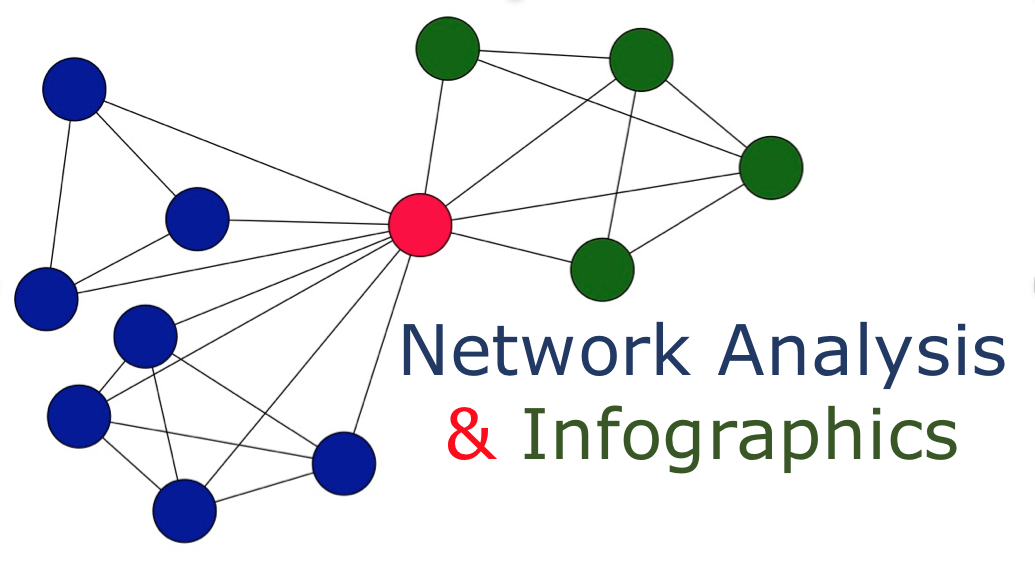
\includegraphics[width=2.5cm]{../_shared_pics/logo}

\medskip

\textit{{\color{dkgreen}{Week 2: 3 February 2022}}}\\
}


\date{} % Date, can be changed to a custom date

\begin{document}

\begin{frame}
\titlepage % Print the title page as the first slide

\begin{textblock*}{10pt}(0pt, 0.9\textheight)

\includegraphics[width=4cm]{../_shared_pics/SPRU.png}
\end{textblock*}

\end{frame}






%=======================================================
%	Intro slides
%=======================================================

\begin{frame}
\frametitle{Overview}
\tableofcontents[hideallsubsections]
\end{frame}

%------------------------------------------------




%=======================================================
%	Ready ...?
%=======================================================
\section*{Ready ...?}

%------------------------------------------------

\bgroup
\setbeamercolor{background canvas}{bg = navyblue}
\begin{frame}[plain]{}
\begin{center}
\color{white}{\Huge\insertsection}
\end{center}
\end{frame}
\egroup


%-----------------------------------

\begin{frame}
\frametitle{\insertsection}
\framesubtitle{R and RStudio}


{\color{blue}{On campus}}
\begin{enumerate}
	\item Go to http://rstudio.uscs.susx.ac.uk/
	\item Access the website by using your University of Sussex account
\end{enumerate}

\medskip

{\color{blue}{On your personal computer}}
\begin{enumerate}
	\item Install R
	\item Install RStudio
\end{enumerate}

\medskip

{\color{blue}{RStudio cloud}}
\begin{enumerate}
	\item Go to \url{https://rstudio.cloud}
	\item Register and sign in
\end{enumerate}

\medskip
\medskip

\end{frame}

%-----------------------------------

\begin{frame}[fragile]
\frametitle{\insertsection}
\framesubtitle{Installing igraph}

Through the {\color{blue}{RStudio interface}}:\\
\begin{enumerate}
	\item Tools
	\item Install Packages
	\item Search for igraph
	\item Tick the box ``Install Dependencies''
	\item Install
\end{enumerate}
\medskip
\medskip
or\\
\medskip
\medskip
Through the {\color{blue}{RStudio console}}

\begin{lstlisting}[language=R]
install.packages("igraph")
library("igraph")
\end{lstlisting}

\end{frame}

%-----------------------------------



%=======================================================
%	R objects
%=======================================================
\section{R objects}

%------------------------------------------------

\bgroup
\setbeamercolor{background canvas}{bg = navyblue}
\begin{frame}[plain]{}
\begin{center}
\color{white}{\Huge\insertsection}
\end{center}
\end{frame}
\egroup

%------------------------------------------------

\begin{frame}
\frametitle{\insertsection}

\begin{itemize}
\item R is an {\color{blue}{object-oriented}} language
\item R creates and manipulate {\color{blue}{objects}}
\item Different types or {\color{blue}{classes}} of objects
\item The most used objects are
    \begin{itemize}
    \item {\color{blue}{Data}} objects    	  
    \item {\color{blue}{Function}} objects
    \end{itemize}
\item Objects have {\color{blue}{attributes}}
\item Objects are stored in a {\color{blue}{workspace}} called \textit{environment} in RStudio
\end{itemize}

\end{frame}

%------------------------------------------------

\begin{frame}
\frametitle{\insertsection}
\framesubtitle{Data objects}

Data \textbf{type}
\begin{itemize}[<+(1)->]
\item {\color{blue}{numeric}}   \\(\textit{1.5, -102, 0.001, ...})
\item {\color{blue}{integer}}   \\(\textit{1, -4, 4, ...})
\item {\color{blue}{character}} \\(\textit{``a'', ``weather'', ``you are'', ...})
\item {\color{blue}{logical}}   \\(\textit{TRUE, FALSE or T, F})
\item ...
\end{itemize}




\end{frame}

%------------------------------------------------

\begin{frame}
\frametitle{\insertsection}
\framesubtitle{Data objects}

\begin{columns}[c]
\column{.6\textwidth}
\begin{minipage}[c][.5\textheight][c]{\linewidth}
	
Data \textbf{structure}
\begin{itemize}[<+(1)->]
\item {\color{blue}{vector}}: an ordered collection of values
\item {\color{blue}{matrix}}: a 2-dimensional vector \\(a vector with $>2$ dimensions is called {\color{blue}{array}})
\item {\color{blue}{data frame}}: variables and observations
\item {\color{blue}{list}}: an ordered sequences of objects
\item {\color{blue}{factor}}: categorical data (e.g.\ ``male'', ``female'')
\end{itemize}

\end{minipage}	   

\column{.4\textwidth}
\begin{minipage}[c][.5\textheight][c]{\linewidth}



\only<2>{
\centering
\footnotesize
\[\mathbf{a} = \left(\begin{array}{@{}c@{}}
0\\
20\\
30\\
-4\\
12\\
\end{array}\right)\]

\[\mathbf{a} = \left(\begin{array}{@{}c@{}}
Peter\\
Sara\\
Andrew\\
Charlotte\\
Rachel\\
\end{array}\right)\]}



\only<3>{
\centering
\footnotesize
\[\mathbf{A} = \left(\begin{array}{@{}ccc@{}}
  0&		10&		20\\
 20&	   -2 &		10\\
 30&	   -10&		5\\
 -4&		 0&		0\\
 12&	   -23&		2\\
\end{array}\right)\]}




\only<4>{
\scriptsize
\centering
\begin{table}
\caption{Students in 2021/22}
\begin{tabular}{lc}
\toprule
\textbf{Student} & \textbf{Course} \\
\hline
Student 1  & SD    \\
Student 2  & STP    	\\
Student 3  & SD    	\\
Student 4  & SIM    \\
Student 5  & SD    \\
Student 6  & STP    \\
Student 7  & SD    \\
Student 8  & SD    	\\
Student 9  & SIM    	\\
Student 10 & SIM    	\\
Student 11 & SD    \\
Student 12 & STP    \\
Student 13 & SD    \\
Student 14 & STP    \\
Student 15 & SD    \\
Student 16 & SIM    \\
Student 17 & SIM    \\
Student 18 & SD    \\
Student 19 & SIM    \\
Student 20 & SIM    \\
\bottomrule
\end{tabular}
\end{table}}

\only<5>{
\centering
\footnotesize

\[\mathbf{a} = \left(\begin{array}{@{}c@{}}
0\\
20\\
30\\
-4\\
12\\
\end{array}\right)\]

\[\mathbf{b} = \left(\begin{array}{@{}c@{}}
red\\
red\\
green\\
yellow\\
yellow\\
\end{array}\right)\]

\[\mathbf{A} = \left(\begin{array}{@{}ccc@{}}
  0&		10&		20\\
 20&	   -2 &		10\\
 30&	   -10&		5\\
 -4&		 0&		0\\
 12&	   -23&		2\\
\end{array}\right)\]}



\only<6>{
\centering
\footnotesize
\[\mathbf{a} = \left(\begin{array}{@{}c@{}}
red\\
red\\
green\\
yellow\\
yellow\\
\end{array}\right)\]

factors	 = green, red, yellow}
\end{minipage}	

\end{columns}


\end{frame}

%------------------------------------------------

\begin{frame}
\frametitle{\insertsection}
\framesubtitle{Functions}

\begin{columns}[c]
\column{.6\textwidth}

\begin{itemize}
\item A {\color{blue}{function}} is a command in R that returns a given outcome
\item Functions can {\color{blue}{read}}, {\color{blue}{manipulate}} and {\color{blue}{analyse}} data
\item Certain {\color{blue}{base functions}} are already integrated in the basic R
\item Packages provide users with {\color{blue}{additional functions}} (e.g.\ igraph)
\end{itemize}
    	   
\column{.4\textwidth}
\footnotesize
\centering

plot()

\medskip

mean()

\medskip

read\_csv(...)

\medskip

write\_csv(...)

...


\end{columns}


\end{frame}

%------------------------------------------------

\begin{frame}
\frametitle{\insertsection}
\framesubtitle{Attributes}

\begin{itemize}
\item {\color{blue}{name}}: the name of the object
\item {\color{blue}{mode}}: the type of data
\item {\color{blue}{length}}: number of elements in the object
\item ..
\end{itemize}

\end{frame}

%------------------------------------------------


%=======================================================
%	R operators
%=======================================================
\section{R operators}

%------------------------------------------------

\bgroup
\setbeamercolor{background canvas}{bg = navyblue}
\begin{frame}[plain]{}
\begin{center}
\color{white}{\Huge\insertsection}
\end{center}
\end{frame}
\egroup

%------------------------------------------------
\begin{frame}
\frametitle{\insertsection}
\framesubtitle{Arithmetic operators}

\centering
\begin{tabular}{cl}
\toprule
\textbf{Operator} & \textbf{Description} \\
\hline
$+$ &         addition\\
$-$ &         subtraction\\
$*$ &         multiplication\\
$/$ &         division\\
$\hat{}$ &    exponentiation\\
\bottomrule
\end{tabular}

\end{frame}

%------------------------------------------------


\begin{frame}
\frametitle{\insertsection}
\framesubtitle{Logical operators}

\centering
\begin{tabular}{cl}
\toprule
\textbf{Operator} & \textbf{Description} \\
\hline
$<$	    	& less than\\
$<=$	    & less than or equal to\\
$>$	    	& greater than\\
$>=$	    & greater than or equal to\\
$==$	    & equal to\\
$!=$	    & not equal to\\
$!x$	    & Not $x$\\
$x \vert y$ & $x$ OR $y$\\
$x \& y$	& $x$ AND $y$\\

\bottomrule
\end{tabular}

\end{frame}

%------------------------------------------------

\begin{frame}
\frametitle{\insertsection}

Let's explore objects and operators in RStudio

\end{frame}

%------------------------------------------------





%=======================================================
% Importing/exporting data in R
%=======================================================
\section{Importing/exporting data in R}

%------------------------------------------------

\bgroup
\setbeamercolor{background canvas}{bg = navyblue}
\begin{frame}[plain]{}
\begin{center}
\color{white}{\Huge\insertsection}
\end{center}
\end{frame}
\egroup

%------------------------------------------------

\begin{frame}
\frametitle{\insertsection}

\begin{itemize}[<+->]
\item R can deal with many different data formats
\item Which data formats do you know?
\item Most commonly used data formats
    \begin{itemize}
    \item {\color{blue}{txt}}: fields are usually separated by \textit{comma}, \textit{tab}, \textit{colon}
    \item {\color{blue}{csv}}: fields are separated by \textit{comma}
    \item {\color{blue}{dta}}: format used by STATA to store data
    \item {\color{blue}{xls/xlsx}}: format used by Excel to store data
    \item ...
    \end{itemize}
\item Text editors: Notepad++ (Windows), TextWrangler (Mac)
\item R packages to read and transform data:
    \begin{itemize}
    \item {\color{blue}{``readr''}} (csv, txt, delimited)
    \item {\color{blue}{``readxl''}} (Excel)
    \item {\color{blue}{``haven''}} (STATA, SPSS, SAS)
    \item {\color{blue}{``tidyverse''}}
    \end{itemize}
\item Install these packages in R (you should now know how to do it)
\end{itemize}

\end{frame}

%------------------------------------------------

\begin{frame}
\frametitle{\insertsection}

Let's import/export data in RStudio

\end{frame}

%------------------------------------------------





%%=======================================================
%	Next time ...
%%=======================================================
\section*{Next time ...}

%------------------------------------------------

\bgroup
\setbeamercolor{background canvas}{bg = navyblue}
\begin{frame}[plain]{}
\begin{center}
\color{white}{\Huge\insertsection}
\end{center}
\end{frame}
\egroup

%------------------------------------------------

\begin{frame}
\frametitle{\insertsection}

\begin{itemize}
\item 	\textbf{Lecture: Network data collection}
	\begin{itemize}
	\item Main approaches to collect and sample network data 
	\item Network boundary specification problem
	\end{itemize}
	
\medskip
\medskip
\item 	\textbf{Seminar: Network data collection}
	\begin{itemize}
	\item Network file formats 
	\item How to create/import and manipulate network data in igraph
	\end{itemize}	

\end{itemize}

\end{frame}

%------------------------------------------------






%%=======================================================
%	Questions
%%=======================================================
\section*{Questions}

%------------------------------------------------

\bgroup
\setbeamercolor{background canvas}{bg = navyblue}
\begin{frame}[plain]{}
\begin{center}
\color{white}{\Huge\insertsection}
\end{center}
\end{frame}
\egroup

%------------------------------------------------




\end{document}